\begin{figure}[t]
  \begin{minipage}{\linewidth}
  \subfloat[Weekday usage is diurnal.]{
  \includegraphics{figures/clients-diurnal-weekday-all}
  \label{fig:weekday-diurnal-all}}\\
  \subfloat[Usage on weekends is more constant.]{
  \includegraphics{figures/clients-diurnal-weekend-all}
  \label{fig:weekend-diurnal-all}}\\
  \caption{Diurnal effect on wireless device usage. There is a clear
    weekday diurnal effect on the number of devices online.}
  \label{fig:diurnal-all}
  \end{minipage}
\end{figure}

\begin{figure}[t]
  \begin{minipage}{\linewidth}
  \subfloat[Upstream traffic, and the measured upstream capacity.]{
  \includegraphics[width=0.98\linewidth]{figures/bitrate_new/diurnal-usage/5_OW4C60DED0F74B_up}
  \label{fig:diurnal-util-uplink-5}}\\
  \subfloat[Downstream traffic, and the measured downstream capacity.]{
  \includegraphics[width=0.98\linewidth]{figures/bitrate_new/diurnal-usage/5_OW4C60DED0F74B_dw}
  \label{fig:diurnal-util-downlink-5}}\\
  \caption{Diurnal pattern of link utilization for one home in our
    deployment.  Capacity remains fairly constant, but utilization
    levels track daily cycles.}
  \label{fig:diurnal-util-5}
  \end{minipage}
\end{figure}

\section{Usage Characteristics}\label{sec:usage}

In this section, we identify notable characteristics of home network usage by
analyzing data from the WiFi, Traffic, and Capacity data sets.
Table~\ref{tab:usage-results} highlights our findings.

\begin{table}[t!]
\begin{small}
\begin{tabular}{|p{2.6in}l|}
\hline
& \\
Weekday traffic is much more diurnal than weekend traffic. &
\S\ref{sec:diurnal}, Fig.~\ref{fig:diurnal-all} \\ & \\
%
Some home networks consistently oversaturate their uplink; they are
likely able to do this because of the ``bufferbloat'' phenomenon. &
\S\ref{sec:saturate}, Fig.~\ref{fig:util-scatter-logx} \\ & \\
%
The single most usage-hungry device consumes about 65\% of the total
home network traffic, on average.  &
\S\ref{sec:device-dist}, Fig.~\ref{fig:passive-device-frac} \\ & \\
%
The most popular domain by volume in a
home network is responsible, on average, for about 38\% of the total wide-area
traffic from that home network, but only 19\% of the connections. &
\S\ref{sec:popular-domains}, Fig.~\ref{fig:passive-domains} \\ & \\
%

\hline
\end{tabular}
\end{small}
\caption{Highlights of Section~\ref{sec:usage} results.}
\label{tab:usage-results}
\end{table}

%\pagebreak{}
\subsection{Which usage patterns are diurnal?}\label{sec:diurnal}
%TODO: rather than usage, isn't this device connectivity? usage seems to imply active data transfer...
Figure~\ref{fig:diurnal-all} uses the WiFi data set to show the mean usage of wireless devices during
each hour of the day, partitioned into weekday (Monday--Friday) and weekend. We
observe a diurnal pattern in the number of unique devices at various times of
day on weekdays; usage peaks during the evenings, and it is lowest during the
afternoons, when users are usually at work.
We see that the number of devices dips only slightly at night
(compared to the dip during the day), which may result from cellular
devices that remain on at night, as opposed to laptops that are more often
switched off at night when users are asleep. Diurnal patterns are less pronounced on weekends.

Figure~\ref{fig:diurnal-util-5} shows an example of diurnal traffic
patterns for upstream and downstream traffic from one home in the 
Traffic data set.  Capacity measurements (shown as the dotted line at the top
of each plot) remains fairly constant, while utilization follows a
roughly diurnal trend.  Many homes in Traffic exhibit patterns
similar to those in Figure~\ref{fig:diurnal-util-5}.

\subsection{Do users saturate their access links?}\label{sec:saturate}
Access link speeds
continue to increase, but it is not known whether users actually take
advantage of this additional capacity.  We measure utilization by computing
the maximum per-second throughput every minute for users in the Traffic
data set. We then compare the 
utilization with the access link throughput as estimated by
Capacity. We only consider instances when there is
some device exchanging traffic with the Internet.
Figure~\ref{fig:util-scatter-logx} plots 95th percentile link
saturation against capacity estimates for uplink and downlink in bits
per second on a log scale.
In most cases there is plenty of spare capacity.
%TODO: some text will change with new figure
At the 95th percentile, only two homes saturate the link and most homes
use less than 50\% of the available capacity.
Thus, even when the link is used, utilization does not come close
to capacity most of the time. If we include cases when the router is on
and connected to the Internet but has no traffic then these numbers drop
even further.

The circles on the scatterplot show the equivalent case for upstream
traffic. We expect upstream usage to be less than downstream, because
popular Internet services download more traffic than they upload; as
expected, upstream utilization is less than downstream.
Figure~\ref{fig:util-scatter-logx} shows that uplink utilization exceeds
capacity for certain homes.  Figure~\ref{fig:over-util-uplink} shows a
timeseries of capacity estimates and utilization for both of these
homes.  This user consistently saturates the uplink; when combined with
``bufferbloat'' problems problems endemic in home networking hardware,
this behavior causes overestimation of the upstream
throughput~\cite{www-bufferbloat}.

\begin{figure}[t]
  \includegraphics[width=0.98\linewidth]{figures/utilization_scatter_v2}
  \caption{Link utilization as a function of the measured throughput.
    Downlink saturation varies between 0 and 1. Uplink saturation is
    under 0.5 for most homes except for 3 cases. 2 homes over utilize
    their uplink} \label{fig:util-scatter-logx}
\end{figure}


\begin{figure}[t]
  \begin{minipage}{\linewidth}
  \subfloat[In this home, utilization always exceeds the measured
    upstream capacity.  Upon further investigation, we discovered that
    this user continually uploads scientific data from his home network.]{
  \includegraphics[width=0.98\linewidth]{figures/bitrate_new/13_OW2CB05D873788_up}
  \label{fig:over-util-uplink-13}}\\
  \subfloat[Diurnal bursts in traffic can sometimes result in
    utilization exceeding the network's upstream capacity.]{
  \includegraphics[width=0.98\linewidth]{figures/bitrate_new/18_OW100D7F64C8A3_up}
  \label{fig:over-util-uplink-18}}\\
  \caption{In some cases, uplink utilization exceeds estimate of
    capacity.  Buffering in customer premises equipment
    (``bufferbloat'') can result in situations where utilization exceeds
  the measured capacity.  These two homes likely experience significant
  latency and performance problems due to constant uplink saturation.}
  \label{fig:over-util-uplink}
  \end{minipage}
\end{figure}

\subsection{How much is each device used?}\label{sec:device-dist}
Figure~\ref{fig:passive-device-frac} shows the fraction
of traffic that individual devices contribute to overall
home data consumption, ordered by the traffic consumption.
%TODO: change text based on new pdf figure for device usage and number of devices per home
%Numbers above the bars indicate how many
%homes have at least that many devices; 
Every household has at least three unique devices, but
 one dominant device typically consumes the bulk of 
the traffic (60\% on average; the next most dominant device consumes
about 20\% of the traffic).
%TODO devices seen by manufacturer grouped plot here - group routers, phones, tablets etc
Although we do not have ground truth about the types of devices in
each home, it is obvious that even if people have
multiple devices, they prefer to consume most data from
a single device.
%TODO which manufacturer is primary device?
Differentiating devices types (\eg, laptops, tablets,
phones, media players, etc.) from network traffic
is ongoing research.

%TODO: replace with pdf for each of 21 homes with num devices on X-axis and device usage fraction on Y-axis
%Now 26 homes
\begin{figure}[t]
  \begin{minipage}{\linewidth}
  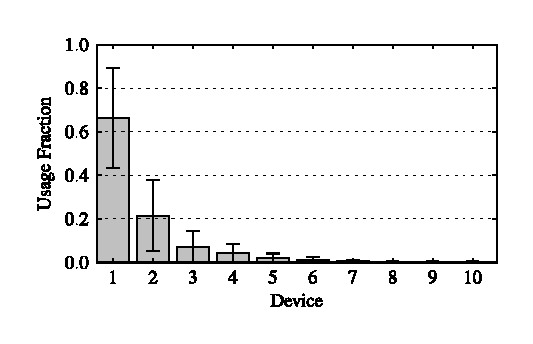
\includegraphics[width=0.98\linewidth]{figures/deviceUtil}
  \caption{Breakdown of data usage by device. We see that even
   in homes with multiple devices, there is usually a dominant
   device responsible for most of the traffic.}
  \label{fig:passive-device-frac}
  \end{minipage}
\end{figure}

%\pagebreak{}
%TODO new plots by Miseon here
\subsection{Which domains receive the most traffic?}\label{sec:popular-domains}

We now examine the popular domains that users in home networks visit
and how those sets of popular domains vary across different home
networks. As described in Section~\ref{sec:data}, we measure statistics
for network traffic to domains that match a whitelist of domain names
based on the 200 most popular domain names from Alexa, plus any domains
that users add to this list using a Web interface built into our router
firmware~\cite{www-alexa-us}. The router anonymizes DNS lookups to all other domains.
%TODO change text based on new plots

\begin{figure}[t]
  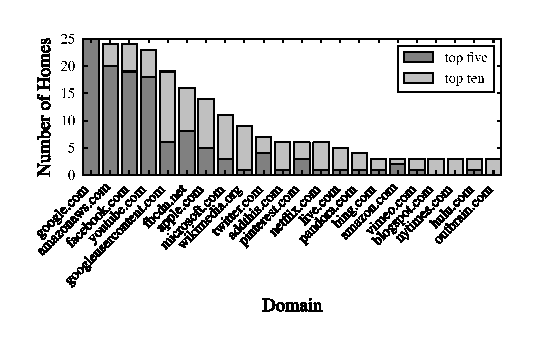
\includegraphics[width=0.98\linewidth]{figures/bytesperdomain/top_five_and_ten_domains}
  \caption{The number of home networks in the Traffic data set for
    which a particular domain appeared in the top-five or top-ten
    domains, ranked by total traffic volume.}
  \label{fig:top-domains}
\end{figure}

\paragraph{Which domains are consistently popular?}
We first explore the domains that are the five and ten
most popular domains in a significant number of home
networks. Figure~\ref{fig:top-domains} shows this distribution; the dark
bar indicates the number of times a particular domain appeared in the top five
domains in a home network, and the lighter bar shows the number of home
networks for which a domain appeared in the top ten.  The most
consistently popular domains on this list are as expected: Google,
YouTube, Facebook, Amazon, Apple, and Twitter.  Unsurprisingly, the
tail is also quite long, with many domains being popular for just one or
two homes (\eg, streaming sites, news sites).  This distribution
confirms on a smaller scale other reports concerning the rise of
``super peers'' who are responsible for sending much of the content into
access networks~\cite{www-sandvine}.


\paragraph{How much traffic are the most popular domains responsible
  for?} 
Figure~\ref{fig:passive-domains} shows the distribution of
domains visited in terms of both total traffic volume and the
number of connections made to the domain (which indicates
the frequency of visits).
Figure~\ref{fig:passive-domains-volume} shows the average
volume of traffic from each home to the most popular domains in the
whitelist.  (We use rank indexes for domains rather than actual names, since
the domain ranking is not exactly the same across all homes.)

The results show that the most popular whitelisted domain by volume on
average accounts for about 38\% of the total traffic volume, even though
these sites are responsible for less than 14\% of connections
(Figure~\ref{fig:passive-domains-volume-conn}); the next most popular
domain accounts for about 11\% of all traffic and only about 7\% of all
connections.  This disproportionality reflects the fact that these
popular domains are most likely serving streaming media content over
long-running TCP connections.  Hence, it is fairly safe to assume that
these top two or three most popular domains by traffic volume are likely
to represent streaming content, which would corroborate other reports
that more than 40\% of traffic into home networks is streaming video
traffic.  Figure~\ref{fig:passive-domains-conn} shows that the domain
with the most number of TCP connections is responsible for about 19\% of
all connections on average; again, this distribution has a very long tail.

It is worth cautioning that our anonymization of some of the domains in
the Traffic data set could bias some of these results.  In
particular, if many homes in our data set for some reason sent a
significant amount of traffic to domains that were not in our whitelist
(\eg, domains for pornographic content, which we explicitly removed from
the whitelist), our results would not reflect this phenomenon.
Nevertheless, because traffic to whitelisted domains represents about
65\% of all traffic volume to and from our home networks on average, we
believe that we have captured a representative sample of usage.
Additionally, the Traffic data set currently only represents homes
in the United States; as we begin to collect this data from home
networks in other countries, we will be able to compare differences in domain
popularity from different home networks.

\begin{figure*}[t]
  \begin{minipage}{\linewidth}
  \subfloat[Distribution of the most popular domains by mean traffic volume.]{
    \includegraphics[width=0.3\linewidth]{figures/volumes_stddev}
  \label{fig:passive-domains-volume}} \hfill
  \subfloat[Distribution of the most popular domains by mean number of connections.]{
  \includegraphics[width=0.3\linewidth]{figures/connections_stddev}
   \label{fig:passive-domains-conn}} \hfill
  \subfloat[Fraction of connections for the most popular domains by volume.]{
  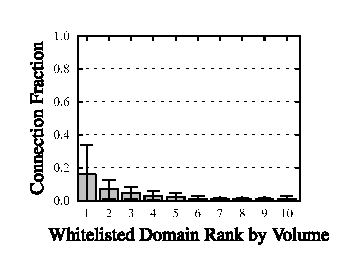
\includegraphics[width=0.3\linewidth]{figures/domain_connection_vs_volume}
  \label{fig:passive-domains-volume-conn}} 
  \caption{Breakdown of data usage by domain.  The
    most popular domain by volume consumes about 38\% of total traffic.
    ``Total'' refers to the portion of traffic to
    whitelisted domains (Alexa top 200, plus any domains that the user
    manually whitelists) and accounts for about 65\% of the total
    traffic on average.}
  \label{fig:passive-domains}
  \end{minipage}
\end{figure*}

\begin{figure}[t]
  \begin{minipage}{\linewidth}
\centering  \subfloat[iMac (Desktop).]{
  \includegraphics[width=0.5\linewidth]{figures/bytesperdomain/d83062e83343-iMac}
  \label{fig:apple-imac}}
\centering  \subfloat[Roku box. ]{
  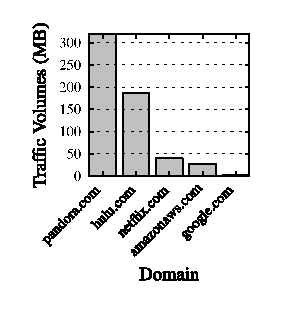
\includegraphics[width=0.5\linewidth]{figures/bytesperdomain/cc6da0849589-Roku}
  \label{fig:roku}}\\
  \caption{Traffic distribution from an Apple iMac (desktop) and a Roku streaming player. 
    For the desktop, Dropbox creates significant traffic to
    {\tt dropbox.com} in the process of syncing large files. The Roku is used almost exclusively for streaming,
    as evidenced by the large fraction of traffic to {\tt pandora.com}, {\tt hulu.com}, and {\tt netflix.com}.}
  \label{fig:apple}
  \end{minipage}
\end{figure}


\paragraph{Do different devices look up different sets of domains?}  We
also examined domain popularity for different devices in home networks,
to see whether the distribution of traffic volumes to domains differed
by device.  Our hypothesis was that certain devices might look up
considerably different sets of domains than others. For example, an
Apple device might exchange more traffic with \url{apple.com}, a
streaming set top box might exchange more traffic with \url{hulu.com},
and so forth.  If true, such a finding could prove extremely valuable
for applications and utilities inside the home that want to
automatically ``fingerprint'' devices---typically, the manufacturer ID
of a device's MAC address may narrow down the device to a manufacturer,
but it is not fine-grained enough to distinguish, say, a laptop from a
smart phone.

To explore this hypothesis, we surveyed users from six homes in the 
Traffic data set and asked them to manually identify the devices
corresponding to each of the MAC addresses in their home.  These labels
provide ground truth identification for these devices.  Here, we show an
example of how different devices send different distributions of traffic
volumes to various domains.  Figures~\ref{fig:apple-imac}
and~\ref{fig:roku} show the distributions for an Apple iMac
Desktop and a Roku Streaming Player, respectively. Whereas a device's MAC address
only reveals the manufacturer, further examination of traffic behavior suggests that
usage patterns may differ significantly enough across {\em types} of devices to serve as
fingerprints for device identification (either automatically, or with
some help from the user).  Exploring how these traffic patterns can
assist with device fingerprinting is an area of future work.



%Figure~\ref{fig:passive-data-util-dw-all}
%plots the same figure for the case that includes durations when the router is
%on but there is no traffic; we see that the link is very rarely used.
%Figure~\ref{fig:passive-data-util-up} shows the equivalent case for upstream
%traffic. We see that the upstream is even more lightly used than
%the downstream. The cases where the utilization is greater than one
%can be explained by buffering in the upstream modem that causes.




%% \begin{figure}[t]
%%   \begin{minipage}{\linewidth}
%%   \subfloat[Downstream]{
%%   \includegraphics[width=0.98\linewidth]{figures/utilization/downlink_utilization}
%%   \label{fig:passive-data-util-dw-active}}\\
%%   \subfloat[Upstream]{
%%   \includegraphics[width=0.98\linewidth]{figures/utilization/uplink_utilization}
%%   \label{fig:passive-data-util-up-active}}\\
%%   \caption{Uplink utilization}
%%   \label{fig:passive-data-util}
%%   \end{minipage}
%% \end{figure}

%TODO: replace with pdf for each of 21 homes with num devices on X-axis and device usage fraction on Y-axis
